\documentclass[11pt,a4paper]{report}

% ---------- PACKAGES ----------
\usepackage[utf8]{inputenc}
\usepackage[T1]{fontenc}
\usepackage{times}
\usepackage[margin=0.9in]{geometry}
\usepackage{graphicx}
\usepackage{tikz}
\usetikzlibrary{shapes.geometric, arrows.meta, positioning, fit, backgrounds}
\usepackage{booktabs}
\usepackage{array}
\usepackage{fancyhdr}
\usepackage{titlesec}
\usepackage{enumitem}
\usepackage{hyperref}
\usepackage{xcolor}
\usepackage{caption}

\setlist{itemsep=1pt, topsep=3pt, parsep=1pt}

\hypersetup{
    colorlinks=true,
    linkcolor=black,
    citecolor=black,
    urlcolor=blue,
    pdftitle={RepairFlow: Right-to-Repair Assistant and Reparability Portal},
    pdfauthor={Punya Chhabra, Arnav Gupta, Kaushik Jindal}
}

% ---------- HEADER/FOOTER ----------


\titleformat{\chapter}[display]
  {\normalfont\Large\bfseries}{\chaptertitlename\ \thechapter}{8pt}{\Large}
\titlespacing*{\chapter}{0pt}{-10pt}{10pt}
\titlespacing*{\section}{0pt}{8pt}{4pt}
\titlespacing*{\subsection}{0pt}{6pt}{3pt}

% Colors for diagram boxes
\definecolor{blueBox}{RGB}{198,217,241}
\definecolor{tealBox}{RGB}{198,235,235}
\definecolor{orangeBox}{RGB}{252,228,178}
\definecolor{redBox}{RGB}{248,206,204}
\definecolor{greenBox}{RGB}{198,239,206}

\begin{document}

% ============================================================
% TITLE PAGE
% ============================================================
\begin{titlepage}
    \centering
    \vspace*{0.3cm}
    {\large UCS503P -- Software Engineering Project\par}
    {\large Academic Year 2026--2027\par}
    \vspace{0.8cm}

    \includegraphics[width=3.5cm]{thapar_logo.png}

    \vspace{0.8cm}

    {\Huge\bfseries RepairFlow: Right-to-Repair\par}
    {\Huge\bfseries Assistant \& Reparability Portal\par}
    \vspace{0.6cm}
    {\Large Repair-Shop Discovery, Request Tracking, and a\par}
    {\Large RAG-Assisted Reparability Portal\par}

    \vspace{1.5cm}

    {\Large\bfseries Submitted by:\par}
    \vspace{0.6cm}

    \begin{tabular}{@{}ll@{}}
        \textbf{1024030684} & Punya Chhabra \\[0.3cm]
        \textbf{1024030780} & Arnav Gupta \\[0.3cm]
        \textbf{1024030431} & Kaushik Jindal \\
    \end{tabular}

    \vspace{1cm}
    {\Large B.E. Third Year, Computer Science \& Engineering\par}

    \vfill

    {\Large\bfseries Submitted to:\par}
    \vspace{0.3cm}
    {\Large\bfseries Dr. Jeelani Asif\par}
    \vspace{0.3cm}
    {\large Department of Computer Science and Engineering\par}

    \vspace{0.8cm}
    {\large\bfseries Mid-Semester Evaluation Report\par}
    \vspace{0.8cm}

    {\large Computer Science and Engineering Department\par}
    {\large Thapar Institute of Engineering and Technology, Patiala\par}

\end{titlepage}

% ============================================================
% TABLE OF CONTENTS
% ============================================================
\tableofcontents
\thispagestyle{empty}
\newpage

% ============================================================
% CHAPTER 1: INTRODUCTION
% ============================================================
\chapter{Introduction}

\section{Background and Context}

When a phone, laptop, or household appliance develops a fault, the owner faces two disconnected problems at once: finding a repair shop that can be trusted with the job, and finding out, before committing to it, whether the fault is even worth repairing. Independent repair shops still rely largely on paper logs and phone calls, so once a device is dropped off there is no way for the owner to check status, cost, or timeline without calling directly. Repair manuals and genuine spare parts are also hard for both owners and shops to source, so perfectly repairable devices are often written off simply because nobody could quickly establish that they were.

This gap has consequences beyond individual inconvenience: global e-waste reached 62 million tonnes in 2022, and only 22\% of it was properly collected and recycled. Right-to-repair legislation -- India's Right to Repair Portal, the EU's repair directive, and new U.S. state laws -- is pushing manufacturers toward repairable design, but legislation alone does not give an owner a fast way to act on it. RepairFlow is proposed as a web platform that closes this gap: an owner describes a device and a fault, is shown repair guidance and a reparability score, and can then discover, request, and track a verified nearby shop through to completion.

\subsection{Problem Statement}

Device owners and independent repair shops lack a single, transparent platform to manage repairs, access parts and documentation, and make repair the easier choice. Owners have no centralised way to discover verified shops or compare quotes; once a device is dropped off there is no visibility into status, cost, or timeline; and slow, opaque repairs push owners toward replacing a device rather than fixing it, adding to the e-waste problem above. RepairFlow addresses this through a RAG-assisted reparability portal combined with a verified-shop directory and an end-to-end request-tracking workflow.

\section{Project Objectives}

The core objectives of the RepairFlow project comprise:

\begin{itemize}
    \item \textbf{Unified Discovery:} Bring device owners, independent repair shops, and reparability information together on one platform.
    \item \textbf{Reparability Guidance:} Surface repair guides and a reparability score for a described device/fault, using a Retrieval-Augmented Generation (RAG) approach over curated documentation.
    \item \textbf{Verified Shop Directory:} List only shops that have passed a verification process, filterable and sortable by rating, distance, and price.
    \item \textbf{End-to-End Tracking:} Let an owner submit a request and follow it through defined status stages, with a ``last updated'' indicator so a stale status is never mistaken for current.
\end{itemize}

% ============================================================
% CHAPTER 2: METHODOLOGY AND DESIGN
% ============================================================
\chapter{Methodology and Design}

\section{System Architecture}

\subsection{High-Level Design}

RepairFlow follows a standard three-tier design: the \textbf{Client Layer}, the \textbf{Application Layer}, and the \textbf{Data Layer}. At this mid-semester stage, the Client Layer has been built as a fully interactive, click-through prototype using static in-browser data, while the Application and Data layers are designed but not yet implemented. Figure 2.1 illustrates the architecture.

\begin{figure}[h!]
\centering
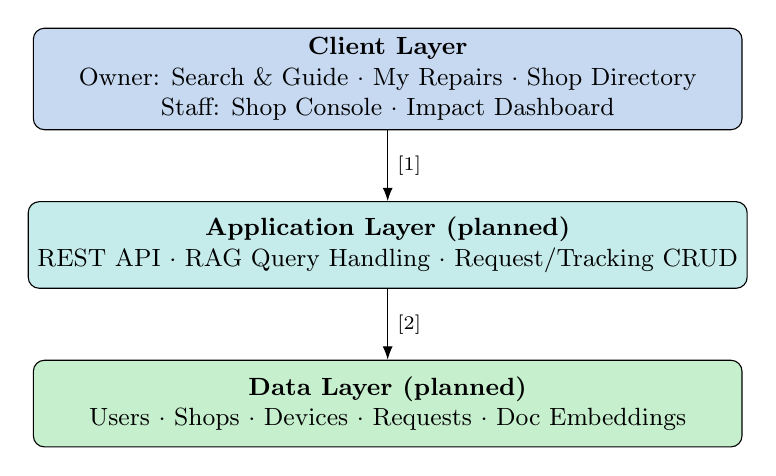
\begin{tikzpicture}[
    box/.style={rectangle, draw, rounded corners, minimum width=9cm, minimum height=1.1cm, align=center, font=\small},
    arrowlabel/.style={font=\scriptsize, align=center}
]
\node[box, fill=blueBox] (client) {\textbf{Client Layer} \\ Owner: Search \& Guide $\cdot$ My Repairs $\cdot$ Shop Directory \\ Staff: Shop Console $\cdot$ Impact Dashboard};
\node[box, fill=tealBox, below=0.9cm of client] (app) {\textbf{Application Layer (planned)} \\ REST API $\cdot$ RAG Query Handling $\cdot$ Request/Tracking CRUD};
\node[box, fill=greenBox, below=0.9cm of app] (data) {\textbf{Data Layer (planned)} \\ Users $\cdot$ Shops $\cdot$ Devices $\cdot$ Requests $\cdot$ Doc Embeddings};

\draw[-{Latex}] (client) -- (app) node[midway, right, arrowlabel] {[1]};
\draw[-{Latex}] (app) -- (data) node[midway, right, arrowlabel] {[2]};
\end{tikzpicture}
\caption{RepairFlow Three-Tier Architecture -- client layer implemented; application and data layers designed and pending}
\end{figure}

The core workflow exercised by the prototype is: an owner describes a device or fault $\rightarrow$ the client matches it against a guide/shop dataset and returns a reparability score, a guide, and a ranked shortlist of verified shops $\rightarrow$ the owner requests a shop and receives a tracking ID $\rightarrow$ the shop updates status and cost, which is reflected immediately back in the owner's tracking view.

\subsection{Technical Stack}

\begin{itemize}
    \item \textbf{Prototype (built):} HTML5, CSS3, and vanilla JavaScript, implemented as a single responsive page with a tab-based router and in-memory state.
    \item \textbf{Planned Backend:} A REST API layer (Spring Boot or an equivalent Node/Express service) handling authentication, request/tracking CRUD, and the shop-verification workflow.
    \item \textbf{Planned Persistence:} A managed relational database for users, shops, devices, and repair requests, alongside a vector store for documentation embeddings used by the RAG pipeline.
    \item \textbf{CI/CD:} A CI runner for build, backend unit tests, and linting on every change, with CD to a staging environment.
    \item \textbf{Version Control:} Git, used to track the prototype and, going forward, the backend implementation.
\end{itemize}

\section{Implementation Details}

\subsection{Module 1: Core Functionality -- Guide Matching \& Shop Discovery}

The Search view is the entry point: an owner types a free-text device/fault description, and a keyword-matching function scores the query against a seeded dataset of four repair guides. The best match populates a repair ``ticket'' card with the device, fault, parts-availability estimate, and a reparability score, and the same query ranks the seeded verified shops to produce a shortlist. Figure 2.2 shows this pipeline.

\begin{figure}[h!]
\centering
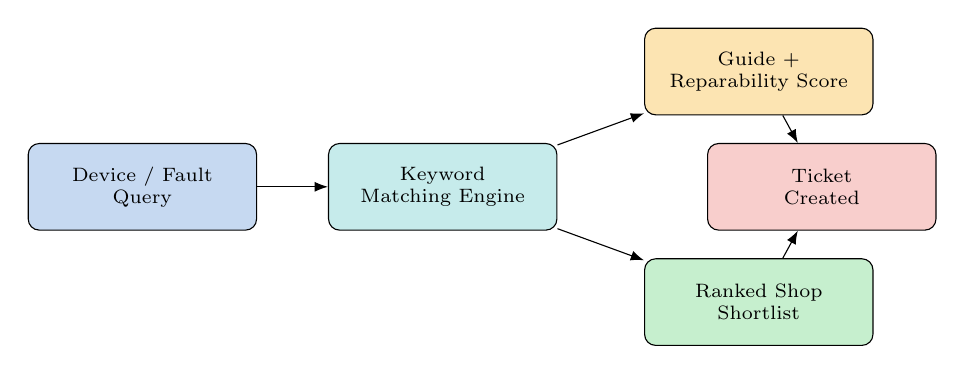
\begin{tikzpicture}[
    node distance=0.5cm and 0.9cm,
    box2/.style={rectangle, draw, rounded corners, minimum width=2.9cm, minimum height=1.1cm, align=center, font=\scriptsize},
    >=Latex
]
\node[box2, fill=blueBox] (n1) {Device / Fault\\Query};
\node[box2, fill=tealBox, right=of n1] (n2) {Keyword\\Matching Engine};
\node[box2, fill=orangeBox, above right=0.35cm and 1.1cm of n2] (n3) {Guide +\\Reparability Score};
\node[box2, fill=greenBox, below right=0.35cm and 1.1cm of n2] (n4) {Ranked Shop\\Shortlist};
\node[box2, fill=redBox, right=1.9cm of n2] (n5) {Ticket\\Created};

\draw[->] (n1) -- (n2);
\draw[->] (n2) -- (n3);
\draw[->] (n2) -- (n4);
\draw[->] (n3) -- (n5);
\draw[->] (n4) -- (n5);
\end{tikzpicture}
\caption{Core Guide-Matching and Shop-Discovery Pipeline}
\end{figure}

This keyword matcher is a deliberate placeholder for the RAG pipeline: it validates the intended contract -- free-text query in, guide plus score out -- before real retrieval and generation are built.

\subsection{Module 2: Secondary Features}

Four further views extend the prototype into the fuller workflow the proposal describes. Figure 2.3 shows how a created ticket flows through the remaining views.

\begin{figure}[h!]
\centering
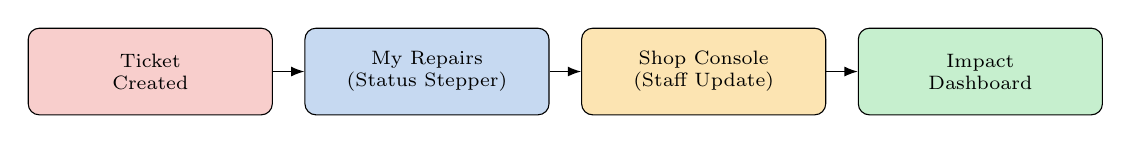
\begin{tikzpicture}[
    node distance=0.4cm and 0.4cm,
    box2/.style={rectangle, draw, rounded corners, minimum width=3.1cm, minimum height=1.1cm, align=center, font=\scriptsize},
    >=Latex
]
\node[box2, fill=redBox] (m1) {Ticket\\Created};
\node[box2, fill=blueBox, right=of m1] (m2) {My Repairs\\(Status Stepper)};
\node[box2, fill=orangeBox, right=of m2] (m3) {Shop Console\\(Staff Update)};
\node[box2, fill=greenBox, right=of m3] (m4) {Impact\\Dashboard};

\draw[->] (m1) -- (m2);
\draw[->] (m2) -- (m3);
\draw[->] (m3) -- (m4);
\end{tikzpicture}
\caption{Secondary Feature Flow: Tracking, Staff Updates, and Sustainability Reporting}
\end{figure}

\begin{itemize}
    \item \textbf{My Repairs:} A five-step status stepper (Submitted $\rightarrow$ Confirmed $\rightarrow$ In progress $\rightarrow$ Ready $\rightarrow$ Closed) per ticket, flagging any open ticket whose ``last updated'' timestamp exceeds 48 hours as ``May be stale.''
    \item \textbf{Shop Directory:} The full seeded shop list, filterable by name/specialty and re-sortable by rating, distance, or price.
    \item \textbf{Shop Console:} A staff-facing table to set a status and cost per ticket; saving writes back into the shared ticket list.
    \item \textbf{Impact Dashboard:} Demo figures for repairs completed and estimated e-waste diverted, shown as placeholders pending real telemetry.
\end{itemize}

% ============================================================
% CHAPTER 3: RESULTS AND EVALUATION
% ============================================================
\chapter{Results and Evaluation}

\section{Testing Methodology}

Because the current build is a client-only prototype, testing at this stage was manual and interaction-driven rather than automated. Each of the five views was exercised directly in the browser: the Search view was tested against all seeded fault categories, the Request $\rightarrow$ My Repairs handoff was checked for correctness, the Shop Console's status/cost edits were confirmed to propagate back into My Repairs, and the 48-hour staleness rule was verified against tickets whose timestamps were deliberately set at 3, 52, and 140 hours old.

\begin{figure}[h!]
\centering
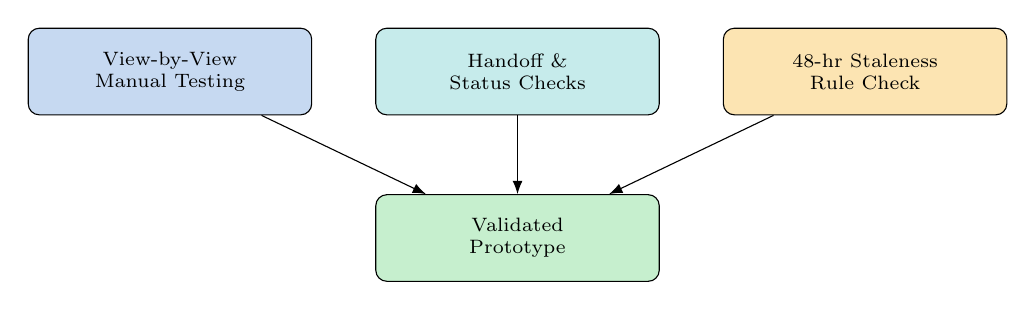
\begin{tikzpicture}[
    box3/.style={rectangle, draw, rounded corners, minimum width=3.6cm, minimum height=1.1cm, align=center, font=\scriptsize},
    >=Latex
]
\node[box3, fill=blueBox] (t1) {View-by-View\\Manual Testing};
\node[box3, fill=tealBox, right=0.8cm of t1] (t2) {Handoff \&\\Status Checks};
\node[box3, fill=orangeBox, right=0.8cm of t2] (t3) {48-hr Staleness\\Rule Check};

\node[box3, fill=greenBox, below=1cm of t2] (t4) {Validated\\Prototype};

\draw[->] (t1) -- (t4);
\draw[->] (t2) -- (t4);
\draw[->] (t3) -- (t4);
\end{tikzpicture}
\caption{Incremental View-by-View Testing Flow}
\end{figure}

\section{Performance Metrics}

The four evaluation metrics defined for the project require a live backend and real user traffic to measure meaningfully; they cannot yet be captured against a static prototype and are therefore reported as pending. Table 3.1 summarises the current status.

\begin{table}[h!]
\centering
\small
\begin{tabular}{p{6.2cm}p{4cm}p{2.8cm}}
\toprule
\textbf{Evaluation Metric} & \textbf{Target Specification} & \textbf{Status} \\
\midrule
Median time-to-answer for a repair query (guides + matching shops) & $\leq$ 3 s & Pending \\
Retrieval relevance rate (queries returning $\geq$ 1 useful guide/shop) & $\geq$ 90\% & Pending \\
Request completion rate (completed vs.\ abandoned/cancelled) & Tracked, no target yet & Pending \\
System uptime during business hours (pilot) & $\geq$ 99\% & Pending \\
\bottomrule
\end{tabular}
\caption{RepairFlow Planned Performance Evaluation Metrics}
\end{table}

\section{Analysis}

The prototype shows that the intended workflow -- describe a fault, receive guidance and a shortlist, request a shop, track it, and roll the outcome into a sustainability figure -- is coherent end to end. The keyword-matching placeholder also gives an early, concrete shape to the RAG pipeline's contract, reducing integration risk once real retrieval and generation are wired in. The remaining work is the Application and Data layers themselves, after which the metrics in Section 3.2 can be measured against real usage.

% ============================================================
% CHAPTER 4: CONCLUSION
% ============================================================
\chapter{Conclusion}

\section{Summary of Work}

This project set out to build RepairFlow, a platform that gives device owners transparent access to repair guidance and verified nearby shops while tracking a repair from request to completion. For this mid-semester stage, the team designed the three-tier architecture proposed at kickoff and implemented a fully interactive client-layer prototype covering guide/shop matching, request creation, status tracking with a staleness safeguard, a browsable verified-shop directory, a staff console, and a sustainability dashboard.

\section{Key Findings}

\begin{itemize}
    \item A small, well-chosen set of fields -- reparability score, parts availability, shop rating/distance/price, and a last-updated timestamp -- is enough to drive the entire owner-facing workflow.
    \item Building the client layer against a static, in-memory dataset before the backend exists validated the full interaction flow early and gives a concrete input/output contract for the RAG pipeline to be built against.
\end{itemize}

\section{Future Work and Recommendations}

For the final project phase, the team will implement:

\begin{itemize}
    \item Build the backend REST API (authentication, request/tracking CRUD, shop verification) and replace the in-memory dataset with a persistent database.
    \item Implement the real RAG pipeline: embed curated repair manuals/guides into a vector store and connect an LLM API call in place of the current keyword matcher.
    \item Implement the shop registration and verification workflow, including lightweight document upload and admin approval.
    \item Wire the CI pipeline (build, backend unit tests, linting) and CD to a staging environment.
\end{itemize}

\section{Final Remarks}

RepairFlow addresses a genuine problem: the absence of a single, transparent place to discover a trustworthy repair shop and know whether a device is worth repairing. The prototype shows the intended owner and shop workflows hold together end to end, on a conventional, deployable stack. What remains is building out the Application and Data layers -- the real API, database, RAG pipeline, and verification workflow -- and then validating accuracy, relevance, and performance at pilot scale.

\end{document}
\documentclass[11pt,a4paper]{report}

% ---------- PACKAGES ----------
\usepackage[utf8]{inputenc}
\usepackage[T1]{fontenc}
\usepackage{times}
\usepackage[margin=0.9in]{geometry}
\usepackage{graphicx}
\usepackage{tikz}
\usetikzlibrary{shapes.geometric, arrows.meta, positioning, fit, backgrounds}
\usepackage{booktabs}
\usepackage{array}
\usepackage{fancyhdr}
\usepackage{titlesec}
\usepackage{enumitem}
\usepackage{hyperref}
\usepackage{xcolor}
\usepackage{caption}

\setlist{itemsep=1pt, topsep=3pt, parsep=1pt}

\hypersetup{
    colorlinks=true,
    linkcolor=black,
    citecolor=black,
    urlcolor=blue,
    pdftitle={RepairFlow: Right-to-Repair Assistant and Reparability Portal},
    pdfauthor={Punya Chhabra, Arnav Gupta, Kaushik Jindal}
}

% ---------- HEADER/FOOTER ----------


\titleformat{\chapter}[display]
  {\normalfont\Large\bfseries}{\chaptertitlename\ \thechapter}{8pt}{\Large}
\titlespacing*{\chapter}{0pt}{-10pt}{10pt}
\titlespacing*{\section}{0pt}{8pt}{4pt}
\titlespacing*{\subsection}{0pt}{6pt}{3pt}

% Colors for diagram boxes
\definecolor{blueBox}{RGB}{198,217,241}
\definecolor{tealBox}{RGB}{198,235,235}
\definecolor{orangeBox}{RGB}{252,228,178}
\definecolor{redBox}{RGB}{248,206,204}
\definecolor{greenBox}{RGB}{198,239,206}

\begin{document}

% ============================================================
% TITLE PAGE
% ============================================================
\begin{titlepage}
    \centering
    \vspace*{0.3cm}
    {\large UCS503P -- Software Engineering Project\par}
    {\large Academic Year 2026--2027\par}
    \vspace{0.8cm}

    \includegraphics[width=3.5cm]{thapar_logo.png}

    \vspace{0.8cm}

    {\Huge\bfseries RepairFlow: Right-to-Repair\par}
    {\Huge\bfseries Assistant \& Reparability Portal\par}
    \vspace{0.6cm}
    {\Large Repair-Shop Discovery, Request Tracking, and a\par}
    {\Large RAG-Assisted Reparability Portal\par}

    \vspace{1.5cm}

    {\Large\bfseries Submitted by:\par}
    \vspace{0.6cm}

    \begin{tabular}{@{}ll@{}}
        \textbf{1024030684} & Punya Chhabra \\[0.3cm]
        \textbf{1024030780} & Arnav Gupta \\[0.3cm]
        \textbf{1024030431} & Kaushik Jindal \\
    \end{tabular}

    \vspace{1cm}
    {\Large B.E. Third Year, Computer Science \& Engineering\par}

    \vfill

    {\Large\bfseries Submitted to:\par}
    \vspace{0.3cm}
    {\Large\bfseries Dr. Jeelani Asif\par}
    \vspace{0.3cm}
    {\large Department of Computer Science and Engineering\par}

    \vspace{0.8cm}
    {\large\bfseries Mid-Semester Evaluation Report\par}
    \vspace{0.8cm}

    {\large Computer Science and Engineering Department\par}
    {\large Thapar Institute of Engineering and Technology, Patiala\par}

\end{titlepage}

% ============================================================
% TABLE OF CONTENTS
% ============================================================
\tableofcontents
\thispagestyle{empty}
\newpage

% ============================================================
% CHAPTER 1: INTRODUCTION
% ============================================================
\chapter{Introduction}

\section{Background and Context}

When a phone, laptop, or household appliance develops a fault, the owner faces two disconnected problems at once: finding a repair shop that can be trusted with the job, and finding out, before committing to it, whether the fault is even worth repairing. Independent repair shops still rely largely on paper logs and phone calls, so once a device is dropped off there is no way for the owner to check status, cost, or timeline without calling directly. Repair manuals and genuine spare parts are also hard for both owners and shops to source, so perfectly repairable devices are often written off simply because nobody could quickly establish that they were.

This gap has consequences beyond individual inconvenience: global e-waste reached 62 million tonnes in 2022, and only 22\% of it was properly collected and recycled. Right-to-repair legislation -- India's Right to Repair Portal, the EU's repair directive, and new U.S. state laws -- is pushing manufacturers toward repairable design, but legislation alone does not give an owner a fast way to act on it. RepairFlow is proposed as a web platform that closes this gap: an owner describes a device and a fault, is shown repair guidance and a reparability score, and can then discover, request, and track a verified nearby shop through to completion.

\subsection{Problem Statement}

Device owners and independent repair shops lack a single, transparent platform to manage repairs, access parts and documentation, and make repair the easier choice. Owners have no centralised way to discover verified shops or compare quotes; once a device is dropped off there is no visibility into status, cost, or timeline; and slow, opaque repairs push owners toward replacing a device rather than fixing it, adding to the e-waste problem above. RepairFlow addresses this through a RAG-assisted reparability portal combined with a verified-shop directory and an end-to-end request-tracking workflow.

\section{Project Objectives}

The core objectives of the RepairFlow project comprise:

\begin{itemize}
    \item \textbf{Unified Discovery:} Bring device owners, independent repair shops, and reparability information together on one platform.
    \item \textbf{Reparability Guidance:} Surface repair guides and a reparability score for a described device/fault, using a Retrieval-Augmented Generation (RAG) approach over curated documentation.
    \item \textbf{Verified Shop Directory:} List only shops that have passed a verification process, filterable and sortable by rating, distance, and price.
    \item \textbf{End-to-End Tracking:} Let an owner submit a request and follow it through defined status stages, with a ``last updated'' indicator so a stale status is never mistaken for current.
\end{itemize}

% ============================================================
% CHAPTER 2: METHODOLOGY AND DESIGN
% ============================================================
\chapter{Methodology and Design}

\section{System Architecture}

\subsection{High-Level Design}

RepairFlow follows a standard three-tier design: the \textbf{Client Layer}, the \textbf{Application Layer}, and the \textbf{Data Layer}. At this mid-semester stage, the Client Layer has been built as a fully interactive, click-through prototype using static in-browser data, while the Application and Data layers are designed but not yet implemented. Figure 2.1 illustrates the architecture.

\begin{figure}[h!]
\centering
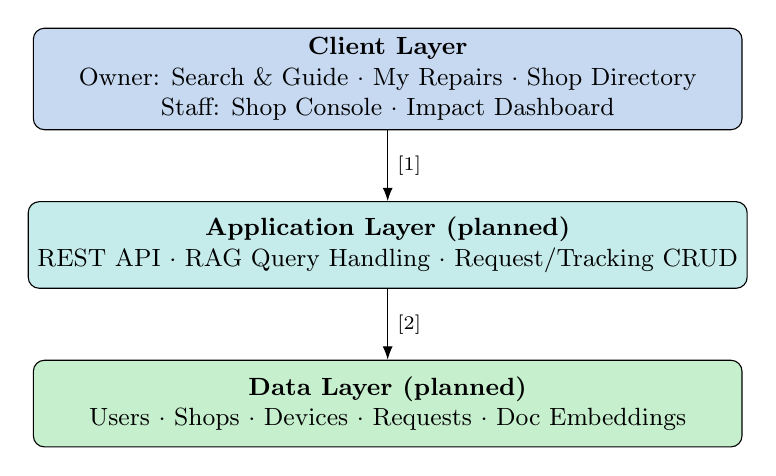
\begin{tikzpicture}[
    box/.style={rectangle, draw, rounded corners, minimum width=9cm, minimum height=1.1cm, align=center, font=\small},
    arrowlabel/.style={font=\scriptsize, align=center}
]
\node[box, fill=blueBox] (client) {\textbf{Client Layer} \\ Owner: Search \& Guide $\cdot$ My Repairs $\cdot$ Shop Directory \\ Staff: Shop Console $\cdot$ Impact Dashboard};
\node[box, fill=tealBox, below=0.9cm of client] (app) {\textbf{Application Layer (planned)} \\ REST API $\cdot$ RAG Query Handling $\cdot$ Request/Tracking CRUD};
\node[box, fill=greenBox, below=0.9cm of app] (data) {\textbf{Data Layer (planned)} \\ Users $\cdot$ Shops $\cdot$ Devices $\cdot$ Requests $\cdot$ Doc Embeddings};

\draw[-{Latex}] (client) -- (app) node[midway, right, arrowlabel] {[1]};
\draw[-{Latex}] (app) -- (data) node[midway, right, arrowlabel] {[2]};
\end{tikzpicture}
\caption{RepairFlow Three-Tier Architecture -- client layer implemented; application and data layers designed and pending}
\end{figure}

The core workflow exercised by the prototype is: an owner describes a device or fault $\rightarrow$ the client matches it against a guide/shop dataset and returns a reparability score, a guide, and a ranked shortlist of verified shops $\rightarrow$ the owner requests a shop and receives a tracking ID $\rightarrow$ the shop updates status and cost, which is reflected immediately back in the owner's tracking view.

\subsection{Technical Stack}

\begin{itemize}
    \item \textbf{Prototype (built):} HTML5, CSS3, and vanilla JavaScript, implemented as a single responsive page with a tab-based router and in-memory state.
    \item \textbf{Planned Backend:} A REST API layer (Spring Boot or an equivalent Node/Express service) handling authentication, request/tracking CRUD, and the shop-verification workflow.
    \item \textbf{Planned Persistence:} A managed relational database for users, shops, devices, and repair requests, alongside a vector store for documentation embeddings used by the RAG pipeline.
    \item \textbf{CI/CD:} A CI runner for build, backend unit tests, and linting on every change, with CD to a staging environment.
    \item \textbf{Version Control:} Git, used to track the prototype and, going forward, the backend implementation.
\end{itemize}

\section{Implementation Details}

\subsection{Module 1: Core Functionality -- Guide Matching \& Shop Discovery}

The Search view is the entry point: an owner types a free-text device/fault description, and a keyword-matching function scores the query against a seeded dataset of four repair guides. The best match populates a repair ``ticket'' card with the device, fault, parts-availability estimate, and a reparability score, and the same query ranks the seeded verified shops to produce a shortlist. Figure 2.2 shows this pipeline.

\begin{figure}[h!]
\centering
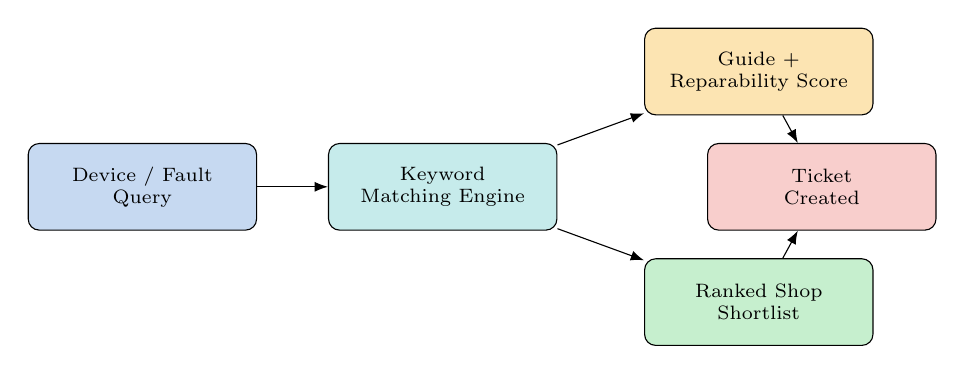
\begin{tikzpicture}[
    node distance=0.5cm and 0.9cm,
    box2/.style={rectangle, draw, rounded corners, minimum width=2.9cm, minimum height=1.1cm, align=center, font=\scriptsize},
    >=Latex
]
\node[box2, fill=blueBox] (n1) {Device / Fault\\Query};
\node[box2, fill=tealBox, right=of n1] (n2) {Keyword\\Matching Engine};
\node[box2, fill=orangeBox, above right=0.35cm and 1.1cm of n2] (n3) {Guide +\\Reparability Score};
\node[box2, fill=greenBox, below right=0.35cm and 1.1cm of n2] (n4) {Ranked Shop\\Shortlist};
\node[box2, fill=redBox, right=1.9cm of n2] (n5) {Ticket\\Created};

\draw[->] (n1) -- (n2);
\draw[->] (n2) -- (n3);
\draw[->] (n2) -- (n4);
\draw[->] (n3) -- (n5);
\draw[->] (n4) -- (n5);
\end{tikzpicture}
\caption{Core Guide-Matching and Shop-Discovery Pipeline}
\end{figure}

This keyword matcher is a deliberate placeholder for the RAG pipeline: it validates the intended contract -- free-text query in, guide plus score out -- before real retrieval and generation are built.

\subsection{Module 2: Secondary Features}

Four further views extend the prototype into the fuller workflow the proposal describes. Figure 2.3 shows how a created ticket flows through the remaining views.

\begin{figure}[h!]
\centering
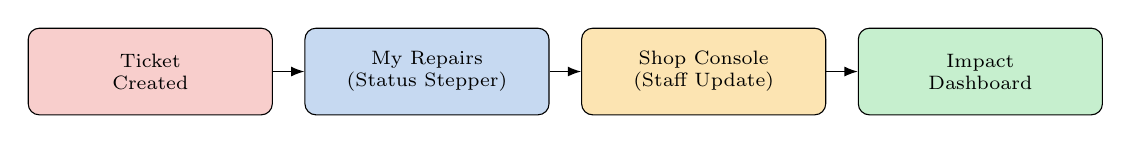
\begin{tikzpicture}[
    node distance=0.4cm and 0.4cm,
    box2/.style={rectangle, draw, rounded corners, minimum width=3.1cm, minimum height=1.1cm, align=center, font=\scriptsize},
    >=Latex
]
\node[box2, fill=redBox] (m1) {Ticket\\Created};
\node[box2, fill=blueBox, right=of m1] (m2) {My Repairs\\(Status Stepper)};
\node[box2, fill=orangeBox, right=of m2] (m3) {Shop Console\\(Staff Update)};
\node[box2, fill=greenBox, right=of m3] (m4) {Impact\\Dashboard};

\draw[->] (m1) -- (m2);
\draw[->] (m2) -- (m3);
\draw[->] (m3) -- (m4);
\end{tikzpicture}
\caption{Secondary Feature Flow: Tracking, Staff Updates, and Sustainability Reporting}
\end{figure}

\begin{itemize}
    \item \textbf{My Repairs:} A five-step status stepper (Submitted $\rightarrow$ Confirmed $\rightarrow$ In progress $\rightarrow$ Ready $\rightarrow$ Closed) per ticket, flagging any open ticket whose ``last updated'' timestamp exceeds 48 hours as ``May be stale.''
    \item \textbf{Shop Directory:} The full seeded shop list, filterable by name/specialty and re-sortable by rating, distance, or price.
    \item \textbf{Shop Console:} A staff-facing table to set a status and cost per ticket; saving writes back into the shared ticket list.
    \item \textbf{Impact Dashboard:} Demo figures for repairs completed and estimated e-waste diverted, shown as placeholders pending real telemetry.
\end{itemize}

% ============================================================
% CHAPTER 3: RESULTS AND EVALUATION
% ============================================================
\chapter{Results and Evaluation}

\section{Testing Methodology}

Because the current build is a client-only prototype, testing at this stage was manual and interaction-driven rather than automated. Each of the five views was exercised directly in the browser: the Search view was tested against all seeded fault categories, the Request $\rightarrow$ My Repairs handoff was checked for correctness, the Shop Console's status/cost edits were confirmed to propagate back into My Repairs, and the 48-hour staleness rule was verified against tickets whose timestamps were deliberately set at 3, 52, and 140 hours old.

\begin{figure}[h!]
\centering
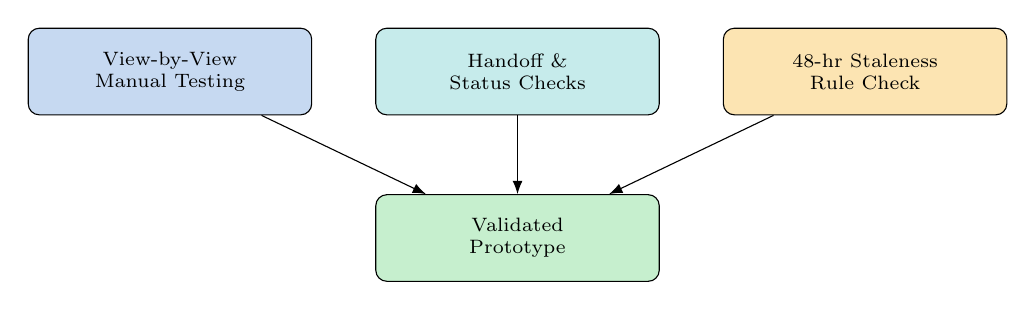
\begin{tikzpicture}[
    box3/.style={rectangle, draw, rounded corners, minimum width=3.6cm, minimum height=1.1cm, align=center, font=\scriptsize},
    >=Latex
]
\node[box3, fill=blueBox] (t1) {View-by-View\\Manual Testing};
\node[box3, fill=tealBox, right=0.8cm of t1] (t2) {Handoff \&\\Status Checks};
\node[box3, fill=orangeBox, right=0.8cm of t2] (t3) {48-hr Staleness\\Rule Check};

\node[box3, fill=greenBox, below=1cm of t2] (t4) {Validated\\Prototype};

\draw[->] (t1) -- (t4);
\draw[->] (t2) -- (t4);
\draw[->] (t3) -- (t4);
\end{tikzpicture}
\caption{Incremental View-by-View Testing Flow}
\end{figure}

\section{Performance Metrics}

The four evaluation metrics defined for the project require a live backend and real user traffic to measure meaningfully; they cannot yet be captured against a static prototype and are therefore reported as pending. Table 3.1 summarises the current status.

\begin{table}[h!]
\centering
\small
\begin{tabular}{p{6.2cm}p{4cm}p{2.8cm}}
\toprule
\textbf{Evaluation Metric} & \textbf{Target Specification} & \textbf{Status} \\
\midrule
Median time-to-answer for a repair query (guides + matching shops) & $\leq$ 3 s & Pending \\
Retrieval relevance rate (queries returning $\geq$ 1 useful guide/shop) & $\geq$ 90\% & Pending \\
Request completion rate (completed vs.\ abandoned/cancelled) & Tracked, no target yet & Pending \\
System uptime during business hours (pilot) & $\geq$ 99\% & Pending \\
\bottomrule
\end{tabular}
\caption{RepairFlow Planned Performance Evaluation Metrics}
\end{table}

\section{Analysis}

The prototype shows that the intended workflow -- describe a fault, receive guidance and a shortlist, request a shop, track it, and roll the outcome into a sustainability figure -- is coherent end to end. The keyword-matching placeholder also gives an early, concrete shape to the RAG pipeline's contract, reducing integration risk once real retrieval and generation are wired in. The remaining work is the Application and Data layers themselves, after which the metrics in Section 3.2 can be measured against real usage.

% ============================================================
% CHAPTER 4: CONCLUSION
% ============================================================
\chapter{Conclusion}

\section{Summary of Work}

This project set out to build RepairFlow, a platform that gives device owners transparent access to repair guidance and verified nearby shops while tracking a repair from request to completion. For this mid-semester stage, the team designed the three-tier architecture proposed at kickoff and implemented a fully interactive client-layer prototype covering guide/shop matching, request creation, status tracking with a staleness safeguard, a browsable verified-shop directory, a staff console, and a sustainability dashboard.

\section{Key Findings}

\begin{itemize}
    \item A small, well-chosen set of fields -- reparability score, parts availability, shop rating/distance/price, and a last-updated timestamp -- is enough to drive the entire owner-facing workflow.
    \item Building the client layer against a static, in-memory dataset before the backend exists validated the full interaction flow early and gives a concrete input/output contract for the RAG pipeline to be built against.
\end{itemize}

\section{Future Work and Recommendations}

For the final project phase, the team will implement:

\begin{itemize}
    \item Build the backend REST API (authentication, request/tracking CRUD, shop verification) and replace the in-memory dataset with a persistent database.
    \item Implement the real RAG pipeline: embed curated repair manuals/guides into a vector store and connect an LLM API call in place of the current keyword matcher.
    \item Implement the shop registration and verification workflow, including lightweight document upload and admin approval.
    \item Wire the CI pipeline (build, backend unit tests, linting) and CD to a staging environment.
\end{itemize}

\section{Final Remarks}

RepairFlow addresses a genuine problem: the absence of a single, transparent place to discover a trustworthy repair shop and know whether a device is worth repairing. The prototype shows the intended owner and shop workflows hold together end to end, on a conventional, deployable stack. What remains is building out the Application and Data layers -- the real API, database, RAG pipeline, and verification workflow -- and then validating accuracy, relevance, and performance at pilot scale.

\end{document}
4
